\documentclass[tikz,border=2mm]{standalone}
\usepackage[thinc]{esdiff}
\begin{document}
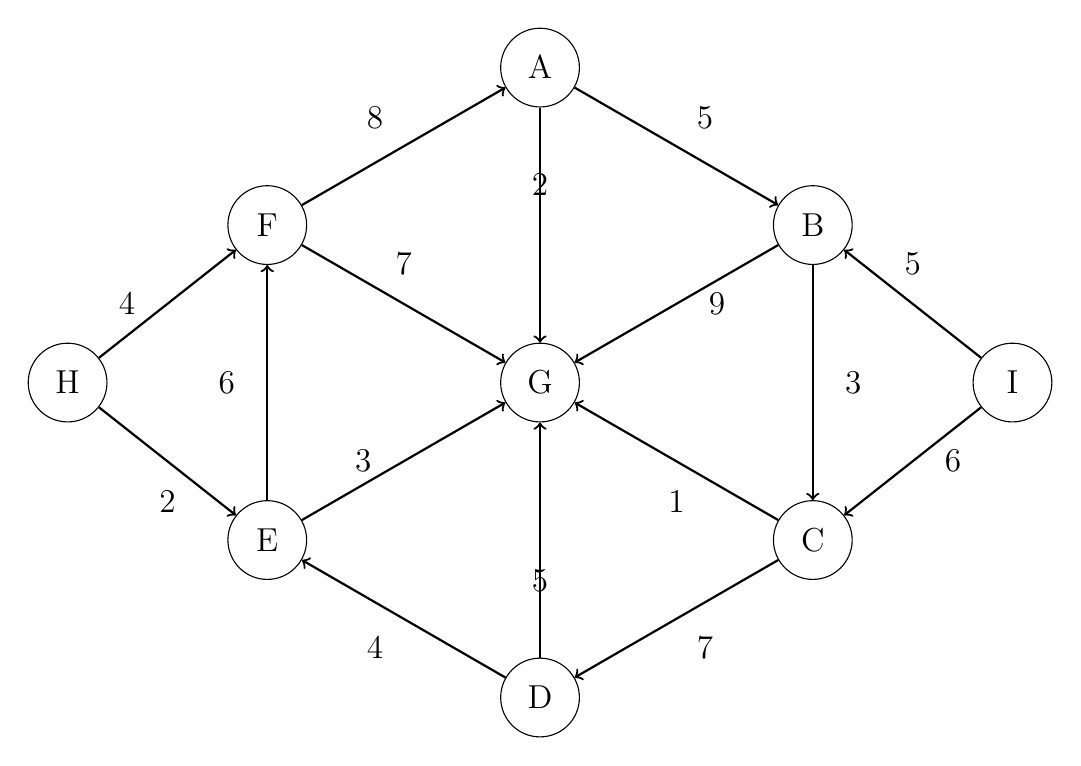
\begin{tikzpicture}[
  node distance=2cm, 
  every node/.style={circle, draw, minimum size=1cm, font=\large}, 
  every label/.style={font=\large}
]

% Nodes arranged in a circle
\node (A) at (90:4cm) {A};
\node (B) at (30:4cm) {B};
\node (C) at (330:4cm) {C};
\node (D) at (270:4cm) {D};
\node (E) at (210:4cm) {E};
\node (F) at (150:4cm) {F};
\node (G) at (0, 0) {G}; % Center node
\node (H) at (180:6cm) {H};
\node (I) at (0:6cm) {I};

% Edges
\draw[->, thick] (A) -- (B) node[midway, above right, draw=none] {5};
\draw[->, thick] (B) -- (C) node[midway, right, draw=none] {3};
\draw[->, thick] (C) -- (D) node[midway, below right, draw=none] {7};
\draw[->, thick] (D) -- (E) node[midway, below left, draw=none] {4};
\draw[->, thick] (E) -- (F) node[midway, left, draw=none] {6};
\draw[->, thick] (F) -- (A) node[midway, above left, draw=none] {8};
\draw[->, thick] (A) -- (G) node[midway, above, draw=none] {2};
\draw[->, thick] (B) -- (G) node[midway, right, draw=none] {9};
\draw[->, thick] (C) -- (G) node[midway, below, draw=none] {1};
\draw[->, thick] (D) -- (G) node[midway, below, draw=none] {5};
\draw[->, thick] (E) -- (G) node[midway, left, draw=none] {3};
\draw[->, thick] (F) -- (G) node[midway, above, draw=none] {7};
\draw[->, thick] (H) -- (F) node[midway, left, draw=none] {4};
\draw[->, thick] (I) -- (C) node[midway, right, draw=none] {6};
\draw[->, thick] (H) -- (E) node[midway, below, draw=none] {2};
\draw[->, thick] (I) -- (B) node[midway, above, draw=none] {5};

\end{tikzpicture}

$$ \diff{}{t} \left[\textrm{O}_3\right] = -k \cdot c (\textrm{CFC}) \cdot c (\textrm{UV})$$

\end{document}
